\documentclass{beamer}
\usepackage[utf8]{inputenc}
\usepackage{graphicx}

\hypersetup{
    colorlinks,%
    citecolor=blue,%
    filecolor=blue,%
    linkcolor=blue,%
    urlcolor=blue 
    %urlcolor=mygreylink     % can put red here to better visualize the links
}

\author[Sowmya Vajjala]{Instructor: Sowmya Vajjala}

\title[LING 520]{LING 520: Computational Analysis of English}
\subtitle{Semester: FALL '16}

\date{27 September 2016}

\institute{Iowa State University, USA}
%%%%%%%%%%%%%%%%%%%%%%%%%%%

\begin{document}

\begin{frame}\titlepage
\end{frame}

\begin{frame}
\frametitle{Class outline}
\begin{itemize}
\item Review of language modeling from thursday's class
\item More on language models
\end{itemize}
\end{frame}

\begin{frame}
\frametitle{Katrin Erk's code}
\begin{itemize}
\item How many of you successfully finished working with Katrin Erk's code samples? What did you understand? \pause
\item How many read Nitin Madnani's article? How many MacOS and Linux users actually tried those terminal commands he showed? \pause
\item How much did you understand from Madnani's article? What did you not understand? \pause
\item What seems to be an easier way to build a simple language model in Python? \pause
\item Did you understand what is "smoothing" and what is "perplexity"? \pause
\item What is "training" and "testing"? \pause
\item Finally, did anyone watch Week 6 lectures by Radev?
\end{itemize}
\end{frame}

\begin{frame}
\frametitle{}
\begin{itemize}
\item If anyone is ready to come and talk about what they learnt from working with Katrin Erk's Python example, they are welcome to do that now. 
\end{itemize}
\end{frame}

\begin{frame}
\frametitle{}
\begin{center}
\Large Quick Recap of Language Modeling basics
\end{center}
\end{frame}

\begin{frame}
\frametitle{Language Model}
\begin{itemize}
\item goal:  predict the next word based on some context. E.g., what is most likely to occur after "Ngram is a sequence of "
\item how do we do?: store frequencies of occurrences of ngram patterns, and calculate the conditional probability of a word occurring given some context of previous words.
\item chain rule of probability for a sentence: 
\begin{itemize}
\item If we assume a sentence S to be a sequence of words (w1, w2, .... wn), then, the probability of this sentence will be:
\item P(S) = p(w1$|$beginning of sentence)*p(w2$|$w1)*p(w3$|$w1,w2)*p(w4$|$w1,w2,w3)*... ... ... *p(wn$|$w1,w2,w3...wn-1)
\end{itemize}
\end{itemize}
\end{frame}

\begin{frame}
\frametitle{The Markov assumption}
\begin{itemize}
\item What is it?: It says instead of computing probabilities using entire history, we can use only the last few previous words.
\item Let us say there is a sentence fragment : "ngram is a sequence of" and we want to estimate the probability of next word being "whatever".
\item P(whatever$|$ngram is a sequence of) can be approximated as P(whatever$|$sequence of) if we choose a trigram model (2 words before current word).
\item P(whatever) - unigram model. P(whatever$|$of) -bigram model .. and so on. 
\end{itemize}
\end{frame}

\begin{frame}
\frametitle{Maximum Likelihood Estimation}
%Copy paste from last week 
\begin{itemize}
\item This is the formula for getting bigram probabilities for one word: P(w$_n|$w$_{n-1}$) = C(w$_{n-1}$,w$_{n}$)/$\Sigma_w$(w$_{n-1}$w) \pause
\item However, $\Sigma_w$(w$_{n-1}$w) just means C(w$_{n-1}$). 
\end{itemize}
\end{frame}

\begin{frame}
\frametitle{Bigram Model Example from J\&M Textbook}
Jurafsky's Language Modeling lecture - slides 16--21.
\end{frame}

\begin{frame}
\frametitle{Major problem with this approach so far}
\begin{itemize}
\item As we discussed last time, most of the bi-gram probabilities are zero. This causes two issues:
\begin{enumerate}
\item Sparse data representation. Solution: Efficient data structures to store data
\item One ngram having a zero probability makes the whole sentence get zero probability.
\end{enumerate}
\item ...and what will we do when we see new words that did not exist in the corpus used to train the language model? 
\item How will we assign probabilities to an unknown event?
\end{itemize}
\end{frame}

\begin{frame}
\frametitle{}
\begin{center}
\Large "Smoothing" in Language Modeling
\end{center}
\end{frame}

\begin{frame}
\frametitle{Smoothing}
\begin{itemize}
\item Used in language model construction to address issues that arise because of having zero probabilities for certain ngrams.
\item intuition: use information about what is known to estimate the unknown.
\item simplest way: start with a count of 1 instead of 0 for everything.
\item better ways: the idea of "discounting" - use the information about ngrams that occur only once or twice in the corpus to estimate frequency of unseen ngrams.
\end{itemize}
\end{frame}

\begin{frame}
\frametitle{Laplace Smoothing/Add one Smoothing}
\begin{itemize}
\item Add 1 to all ngram counts in the model - this ensures we never get a non-zero probability.
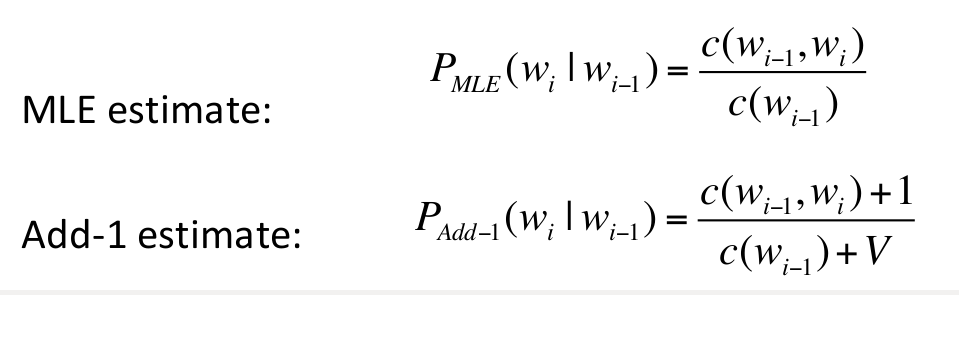
\includegraphics[width=0.9\textwidth]{add1.png}
\item We never assign a zero count to any ngram in this. We start with 1.
\end{itemize}
\end{frame}

\begin{frame}
\frametitle{Handling Unknown, Out of vocabulary words}
\begin{itemize}
\item What if we actually see a word that was never seen in training in the first place? \pause
\item Typically, such situations are handled in two ways:
\begin{itemize}
\item Split the training set into two parts, and replace all words in part 2 that are not seen in part 1 as $<UNK>$. Use that as a proxy for any new word you see in test data.
\item Replace the first occurrence of any word in training set with $<UNK>$ and develop the model. Replace any new word in test data with $<UNK>$ and test.
\end{itemize}
\end{itemize}
\end{frame}

\begin{frame}
\frametitle{Backoff and Interpolation}
%Talk about zero probabilities issue
\begin{itemize}
\item Back-off: If a trigram in the test sentence is not seen in training data, back off to the bigram probabilities. If a bigram is also not seen, back off to unigram model. 
\item When we back-off, we take a discounted version of the lower order ngram probability.
\item Interpolation: If let us say I have a trigram model. Then, I use uni, bi, trigrams to estimate probabilities, by assigning weights to these.
\item E.g., in interpolated LM, P(test\_sentence) = weight1*trigram\_prob + weight2*bigram\_prob + weight3*unigram\_prob
\end{itemize}
(Note: Discussion about their implementation is beyond the scope of this course. Read Chapter 4 in J\&M)
\end{frame}

\begin{frame}
\frametitle{Advanced Smoothing Methods}
\begin{itemize}
\item Good-Turing discounting
\item Witten-Bell discounting
\item Kneser-Ney smoothing
\item Class based ngrams (based on grouping similar ngrams)
\end{itemize}
(Note: Discussion about their working is beyond the scope of this course. Read Chapter 4 in J\&M)
\end{frame}

\begin{frame}
\frametitle{}
\begin{center}
\Large Evaluating a Language Model
\end{center}
\end{frame}

\begin{frame}
%Extrinsic and Intrinsic Evaluation
\frametitle{What is evaluation for a language model?}
\begin{itemize}
\item How good is our model at assigning higher probabilities to well formed sentences?
\item Is the model giving low probability to unlikely sentence constructions?
\item We "train" the parameters of our language model (probabilities) using a large corpus, called "Training set"
\item We test how the model is doing with a new set of sentences called "Test set"
\item We use some evaluation metric to judge the model performance, after looking at how the model does with test set.
\end{itemize}
\end{frame}

\begin{frame}
\frametitle{Training and Test Set}
\begin{itemize}
\item Training set: the corpus of sentences we use to develop our language model.
\item Test set: the corpus of sentences we use to evaluate of the model.
\item Sometimes, there is also an initial test set called "development set" which you use to do preliminary evaluations, and finally test on the actual test-set.
\item If there is a corpus of 100K sentences, generally, we use 80K for training, 10K for development, 10K for testing.
\item Bad science: using the same data for training and testing. 
\end{itemize}
\end{frame}

\begin{frame}
\frametitle{Extrinsic and Intrinsic Evaluation}
\begin{itemize}
\item Best way to evaluation one language model against another is to put it to use for some task (speech recognition, grammatical error correction etc)
\item Get the accuracy for that task for model A and model B and decide which is the better model for that task.
\item Drawback: Expensive and time consuming too. 
\item Solution: Do intrinsic evaluation using small test sets. This is good only for pilot experiments and initial research. Not for deciding about actual usage in a real application. 
\end{itemize}
\end{frame}

\begin{frame}
\frametitle{Intrinsic Evaluation of Language Models}
\framesubtitle{Perplexity and Log Probability}
\begin{itemize}
\item Perplexity is given by the formula: P(w$_1$,w$_2$...w$_n$)$^{-1/N}$ where N is the number of tokens in the sentence.
\item Madnani's article represents Perplexity interms of log probability. Mathematically both these representations are the same (Derive yourself if interested!).
\item Minimizing perplexity == Maximizing the probability of a sentence. \pause
\item Why is taking a logarithm of probability useful instead of normal probability? \pause
\item log(0.00000000000000001) = -17 (Such extremely small or extremely large values are easy to interpret and compare on log scale).
\item Also, log(a*b) = log(a) + log (b). Adding is faster than multiplying computationally.
\end{itemize}
\end{frame}

\begin{frame}
\frametitle{Using perplexity in real experiments - 1}
\begin{itemize}
\item Scenario 1: I trained three language models  (1 unigram, 1 bigram and 1 trigram) using all texts written by Shakespeare. 
\item Now, I have a newly discovered Shakespearean text and I want to find out how close it is to these models. 
\item The perplexity scores of these 3 language models for this text are (450, 200, 120).
\item Which is the better model to represent my new text? \pause
\item The model with lower perplexity is always a better model.
\item If we expect our training data and test data to have the same style of word usage and so on, a trigram model is always better than a bigram model, which is always better than a unigram model.
\end{itemize}
\end{frame}

\begin{frame}
\frametitle{Using perplexity in real experiments - 2}
\begin{itemize}
\item Let us say I want to understand whether English writing of Chinese learners is closer to Korean learners or to German learners.
\item I train one language model for Korean learner corpus, one language model for German learner corpus.
\item Now, give some Chinese learner writing to both these models and get a perplexity score.
\item If perplexity of Korean model is 100, and perplexity of German model is 200, we can conclude: Chinese learner's English writing is closer to Korean learner's English writing compared to German learners. 
\end{itemize}
\end{frame}

\begin{frame}
\frametitle{Using perplexity in real experiments - 3}
Important thing to note: Perplexity score as a standalone number does not mean anything. It can only be used to compare between models. 
\end{frame}

\begin{frame}
\frametitle{Training and Storing Language Models}
\begin{itemize}
\item Katrin Erk's example shows how to build simple and small language models in Python.
\item Some common toolkits to train large, and storage efficient language models: SRILM, CMULM, KenLM, Kylm etc.
\item They all expect corpus to be in: one line per sentence, tokens seperated by whitespace format.
\item Trained model is stored in a format called ARPA, which stores 1--N gram log probabilities, along with Backoff weights and other such necessary stuff.
\item The toolkits support various smoothing methods, and other optimization options.
\item Madnani's article tells how to use these in Python.
\item Other ways of training LM: Use POS tag ngrams, Word-POS tag combos, Phrase ngrams etc.
\end{itemize}
\end{frame}

\begin{frame}
\frametitle{Some relevant resources}
\begin{itemize}
\item Google Ngram viewer: \url{https://books.google.com/ngrams} (and a criticism: \url{https://goo.gl/LwE7cn})
\item Python libraries to use pre-existing language models: 
\begin{enumerate}
\item \url{https://pypi.python.org/pypi/arpa/0.1.0b1}
\item \url{https://github.com/awni/py-arpa-lm} 
\end{enumerate}
\item SRILM: \url{http://www.speech.sri.com/projects/srilm/}
\item CMULM: \url{http://www.speech.cs.cmu.edu/SLM/toolkit.html}
\item KenLM: \url{https://kheafield.com/code/kenlm/}
\item KyLM: \url{http://www.phontron.com/kylm/}
\end{itemize}
\end{frame}

\begin{frame}
\frametitle{Practice Exercise}
Modify Katrin Erk's code sample to incorporate Laplace smoothing and return Log probabilities instead of normal probability.
\\Note: This is going to be useful in doing Question 1 of Assignment 3. So, try to do this.
\end{frame}

\begin{frame}
\frametitle{Next Class}
\begin{itemize}
\item Topics: POS Tagging Introduction, Assignment 2 discussion, Assignment 3 description
\item ToDo: Submit Assignment 2
\end{itemize}
\end{frame}
\end{document}



